\def\QRCODE{MASTER_mispa_TUT.IMG.lip_pythonqrcode.png}
\def\QRPAGE{http://www.iptutorials.science/tree/master/MASTER_mispa/TUT.IMG.lip/python}
\pcorrectionsection{Python correction}

\subsection{Elementary operations}
The most important function to code is the graytone transformation function. It
considers M as the maximum value (the absolute white). This code means that
the absolute white cannot be reached, and thus $f\in[0; M[$. After discretizing the gray values, $F\in[0; M-1]$.

\begin{python}
"""
file LIP.py
LIP simple module
USAGE: import LIP

"""
import numpy as np

def graytone(F, M):
    # graytone function transform
    # M: maximal value
    # F: image function
    f = M-np.finfo(float).eps-F;
    return f;
\end{python}
\begin{python}    
def phi(f, M):
    # LIP isomorphism
    # f: graytone function
    # M: maximal value
    l = -M * np.log(-f/M+1);
    return l
\end{python}
\begin{python}    
def invphi(l, M):
    # inverse isomorphism
    f = M*(1-np.exp(-l/M));
    return f
\end{python}
\begin{python}
def plusLIP(a, b, M):
    # LIP addition
    z = a+b-(a*b)/M;
    return z;
\end{python}
\begin{python}
def timesLIP(alpha, x, M):
    # LIP multiplication by a real
    z = M-M*(np.ones(x.shape)-x/M)**alpha;
    return z;
\end{python}

\subsection{LIP dynamic expansion}
The optimal value for dynamic expansion is given by $\lambda_0$:
$$\lambda_0(f)=\arg\max_{\lambda}\left\{\max(\lambda\lipfois{} f)-\min(\lambda\lipfois{} f) \right\}$$

Let $A(\lambda)=\max(\lambda\lipfois{} f)-\min(\lambda\lipfois{} f)=\lambda\lipfois{}\max(f)-\lambda\lipfois{}\min(f)$ and $B=\ln(1-\min(f)/M)$ et $C=\ln(1-\max(f)/M)$.\vspace*{-1.2\baselineskip}


\begin{eqnarray*}
A'(\lambda)=0&\Leftarrow &[(M-M\exp(\lambda C))-(M-M\exp(\lambda B))]'=0\\
&\Leftarrow & [\exp(\lambda B)-\exp(\lambda C)]'=0\\
&\Leftarrow & B\exp(\lambda B)-C\exp(\lambda C)=0\\
&\Leftarrow & \ln(B)+\lambda B=\ln(C) -\lambda C\\
&\Leftarrow & \lambda=\frac{\ln(C)-\ln(B)}{B-C}\\
&\Leftarrow & \lambda=\frac{\ln(C/B)}{B-C}
\end{eqnarray*}
Thus, yielding to:
$$\lambda_0(f)=\frac{\displaystyle\ln\left(\frac{\ln(1-\max(f)/M)}{\ln(1-\min(f)/M)}\right)}{\displaystyle\ln\left(\frac{M-\min(f)}{M-\max(f)}\right)}$$

This is coded in python by:

\begin{python}
def computeLambda(f, M):
    # compute optimal value for dynamic expansion
    B = np.log(1-f.min()/M);
    C = np.log(1-f.max()/M);
    l = np.log(C/B)/(B-C);
    return l;
\end{python}

\vspace*{-.5\baselineskip}

\subsection{Complete code}
This code uses a transform called histogram equalization. This version proposes our own code for the histogram equalization \iflabelexists{tutorial:image_enhancement}{ (see also \ref{tutorial:image_enhancement}}{(see introduction tutorial on image enhancement)}.
\begin{python}
import LIP
import numpy as np
from scipy import misc
import matplotlib.pyplot as plt
import skimage
""" Histogram equalization
"""
def histeq(im,nbr_bins=256):
   #get image histogram
   imhist,bins = np.histogram(im.flatten(),nbr_bins,normed=True)
   cdf = imhist.cumsum() #cumulative distribution function
   cdf = 255 * cdf / cdf[-1] #normalize
   #use linear interpolation of cdf to find new pixel values
   im2 = np.interp(im.flatten(),bins[:-1],cdf)

   return im2.reshape(im.shape), cdf
\end{python}

It is compared to the LIP dynamic enhancement. The results are illustrated in Fig. \ref{lippython:fig:enhancement}.

\begin{python}
M = 256.

# reads original image
B = imageio.imread("breast.jpg");

# conversion to gray-tones (see LIP definition)
tone = LIP.graytone(B, M);
D = LIP.graytone(LIP.timesLIP(.5, tone, M), M);

# compute optimal enhancement value
l = LIP.computeLambda(tone, M);
print "lambda: %f" % l
# apply enhancement and get back into classical space
E = LIP.graytone(LIP.timesLIP(l, tone, M), M);

# histo equalization, for comparison purposes
heq,cdf = histeq(B);

# display results
plt.figure();
plt.subplot(1,3,1); plt.imshow(E/M, cmap=plt.cm.gray, vmin=0, vmax=1); plt.title('dynamic expansion');
plt.subplot(1,3,2); plt.imshow(B/M, cmap=plt.cm.gray, vmin=0, vmax=1); plt.title('original image');
plt.subplot(1,3,3); plt.imshow(heq/M, cmap=plt.cm.gray, vmin=0, vmax=1); plt.title('after histo equalization');
\end{python}

\begin{figure}[htbp]
\centering\caption{Comparison of the LIP enhancement with the classical histogram equalization method.}%
 \subfloat[Original image]{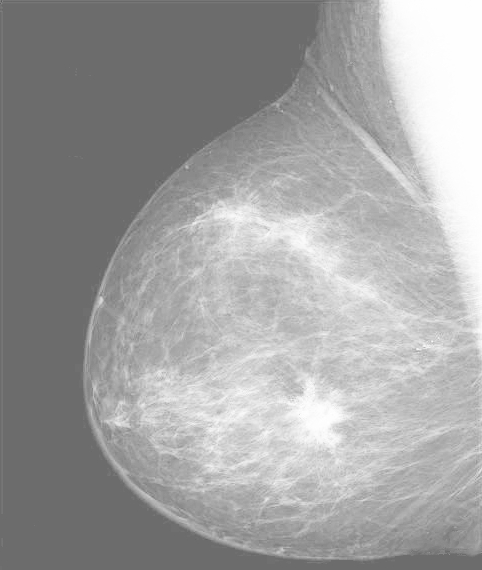
\includegraphics[width=4.7cm]{breast.jpg}} \hspace{.5cm}
 \subfloat[LIP enhancement.]{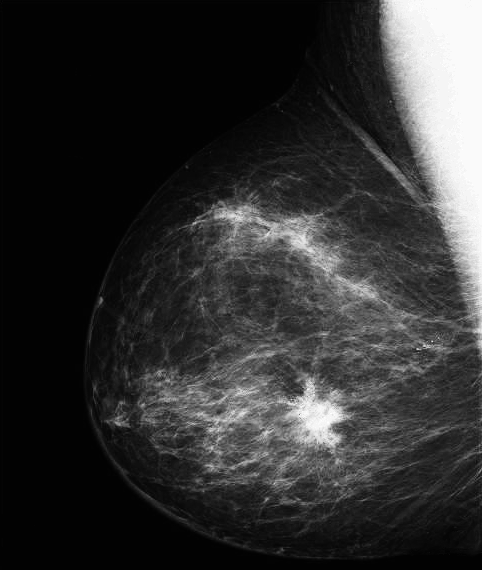
\includegraphics[width=4.7cm]{lipenhance.png}}\hspace{.5cm}
 \subfloat[Histogram equalization.]{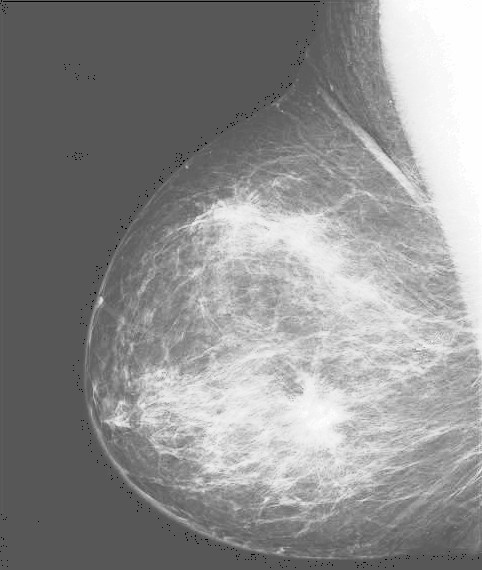
\includegraphics[width=4.7cm]{histeq.png}}%
 \vspace*{-3mm}%
 \label{lippython:fig:enhancement}%
\end{figure}

\subsection{Edge detection}
When applying an operator in the LIP framework, it is better to apply first the
isomorphisme, then the operator, and then get back into the classical space. This
is applied for example for an edge detection operator.

The method applied here is the Sobel gradient. The results are presented in Fig. \ref{lippython:fig:sobel}.

\begin{python}
# contours detection
# Sobel detection
def Sobel(I):
    sobx=cv2.Sobel(I, -1, 1, 0);
    soby=cv2.Sobel(I, -1, 0, 1);
    sob = np.sqrt(sobx**2 + soby**2);
    return sob;

# go into LIP space
tonelip = LIP.phi(tone, M);

# apply Sobel filter
sobellip = LIP.graytone(LIP.invphi(Sobel(tonelip), M), M);
imageio.imwrite("sobellip.png", sobellip);
plt.figure();
plt.subplot(1,2,1);plt.imshow(sobellip, cmap=plt.cm.gray); 
plt.title('LIP Sobel edge detection')

# apply Sobel filter in the classic space
sobel = 255-Sobel(B);
plt.subplot(1,2,2); plt.imshow(sobel, cmap=plt.cm.gray); 
plt.title('Sobel edge detection')
imageio.imwrite("sobel.png", sobel);
\end{python}

\begin{figure}[htbp]
\centering\caption{Sobel edge detection}%
\subfloat[LIP Sobel edge detection.]{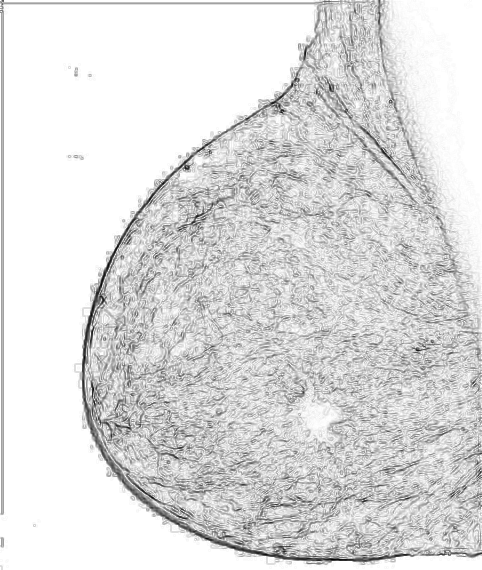
\includegraphics[width=4.7cm]{sobellip.png}}\hspace{1cm}
\subfloat[Classic Sobel edge detection.]{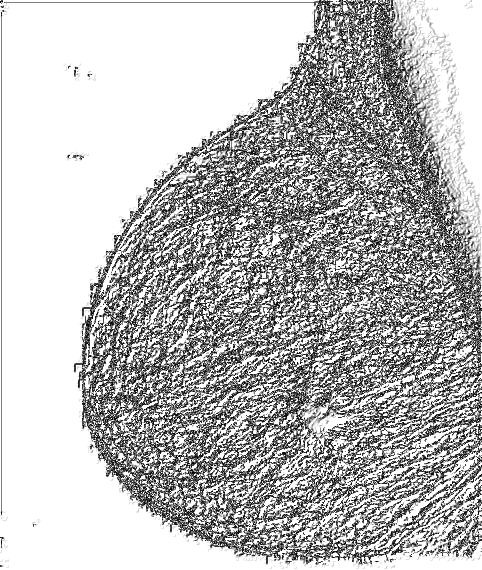
\includegraphics[width=4.7cm]{sobel.png}}%
\vspace*{-3mm}%
\label{lippython:fig:sobel}%
\end{figure}
